% !TeX spellcheck = id_ID
\documentclass[a4paper,12pt]{article}
\usepackage[bahasa]{babel}
\usepackage{graphicx}
\usepackage{multirow}
\usepackage{enumitem}
\usepackage{listings}
\usepackage{wrapfig}
\usepackage[T1]{fontenc}
\usepackage{inconsolata}
\usepackage{lipsum}
\usepackage{adjustbox}


\usepackage{color}
\usepackage[table]{xcolor}
\definecolor{pblue}{rgb}{0.13,0.13,1}
\definecolor{pgreen}{rgb}{0,0.5,0}
\definecolor{pred}{rgb}{0.9,0,0}
\definecolor{pgrey}{rgb}{0.46,0.45,0.48}
\lstset{language=Java,
	showspaces=false,
	showtabs=false,
	breaklines=true,
	showstringspaces=false,
	breakatwhitespace=true,
	commentstyle=\color{pgreen},
	keywordstyle=\color{pblue},
	stringstyle=\color{pred},
	rulecolor=\color{black},
	basicstyle=\ttfamily,
	moredelim=[il][\textcolor{pgrey}]{$$},
	moredelim=[is][\textcolor{pgrey}]{\%\%}{\%\%}
}

\graphicspath{ {./img/} }
\begin{document}
\title{ {\Large Laporan Praktikum}\\ Algoritma dan Pemrograman \\{\Large Pertemuan 12}}

\author{Aldzikri Dwijayanto Prathama 
	\\195410189
	\\Teknik Informatika}
\makeatletter
\begin{titlepage}
	\begin{center}
		{\huge \bfseries \@title }\\[14ex]
		
\includegraphics[scale=.8]{logo}\\[4ex]
		{\large \@author}\\[19ex]
		{\large \bfseries {SEKOLAH TINGGI MANAJEMEN INFORMATIKA DAN KOMPUTER
				AKAKOM YOGYAKARTA}}
	\end{center}


%{\large \@date} 
\end{titlepage}
\makeatother
%\maketitle
\newpage
\tableofcontents
\newpage

\section{Tujuan}
Mahasiswa dapat mengimplementasikan konsep perulangan while untuk menyelesaikan kasus

\section{Dasar Teori}
\paragraph{}
Pada dasarnya sebuah program dieksekusi secara runtut dari mulai statement yang
pertama kali dibaca dilanjutkan dengan statement yang dibaca berikutnya.
Tetapi alur pemrosesan itu bisa diubah dengan menggunakan seleksi dan
perulangan sehingga memungkinkan sebuah program menjalankan tugas yang lebih
kompleks.
Alur pemrosesan dimulai dari bagian utama program.
\begin{itemize}[label=*.] 
    \item Seleksi dan iterasi/perulangan dapat digabungan dengan dua kemungkinan,
    yang pertama seleksi dalam perulangan dan yang kedua adalah perulangan
    dalam seleksi (akan dibahas pada pertemuan ke-13), gambaran sederhana dari
    model yang pertama adalah:
    \begin{lstlisting}[frame=single]
        for(ungkapan1;ungkapan2;ungkapan3)
        {
            if(kondisi)
            {
                Statement;
            }
        }
    \end{lstlisting}
\end{itemize}
Keterangan
\begin{itemize}[label=*.]
    \item Dalam model ini, statement baru akan dijalankan jika kondisi dalam if bernilai
benar. Statement akan terus dijalankan selama ungkapan2 dalam for masih
bernilai benar.
\end{itemize}
\newpage
\section{Praktik}
\subsection{Praktik 1}
Ketik dan amati hasil output dari program berikut ini\\
\begin{center}
    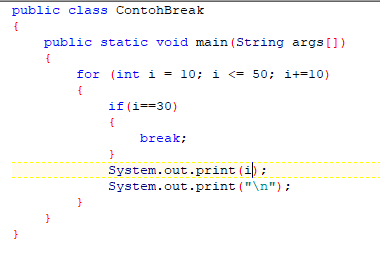
\includegraphics[scale=1]{image1}
\end{center}
Pada program di atas terdapat perulangan for, yang nilai memiliki nilai variabel i 10, perulangan ini akan terus berjalan selama variabel i lebih kecil sama dengan 50, dan variabel i akan bertambah 10 di setiap perulangan.\\
Lalu di dalam perulangan tersebut terdapat seleksi dengan kondisi 1 = 30, dengan pernyataan break;. Jadi jika variabel i bernilai 30, maka perulangan akan berakhir.\\
Jadi jika program tersebut dijalankan akan mengeprint bilangan 10 dan 20 ke layar seperti di bawah\\
\begin{center}
    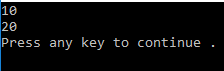
\includegraphics[scale=1]{image2}
\end{center}

\subsection{Praktik 2}
Ketik dan amati hasil output dari program berikut ini\\
\begin{center}
    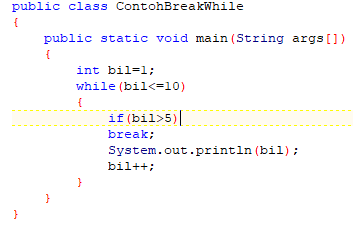
\includegraphics[scale=1]{image3}
\end{center}
Program di atas memiliki variabel bil bernilai 1, lalu perulangan while yang akan berjalan jika variabel bil lebih kecil dari sama dengan 10. Didalamnya terdapat seleksi yang memiliki kondisi bil>5 dan pernyataan break. Jadi program akan mengeprint bilangan 1 - 5 ke layar seperti berikut.
\begin{center}
    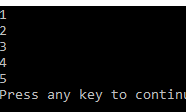
\includegraphics[scale=1]{image4}
\end{center}

\subsection{Praktik 3}
Cobalah program di bawah, jalankan dan amati hasilnya\\
\begin{center}
    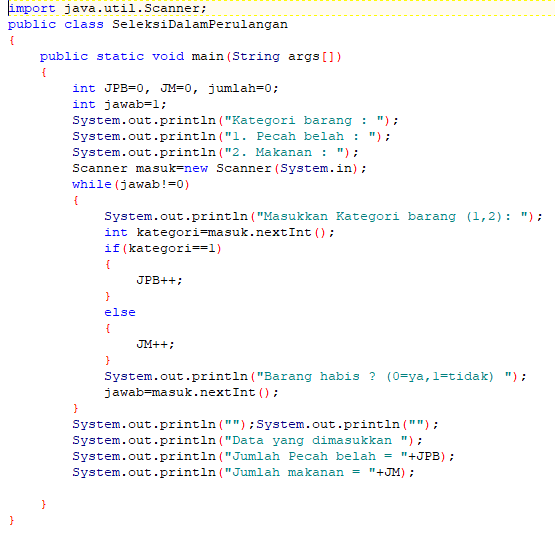
\includegraphics[scale=.8]{image5}
\end{center}
Program di atas memiliki perulangan while yang akan berjalan selama variabel jawab bernilai selain 0. Di dalam perulangan tersebut terdapat seleksi if yang memiliki kondisi kategori == 1 dan memiliki pernyataan JPB++, jadi seleksi ini akan menambahkan nilai satu ke variabel JPB jika kondisi bernilai true. Lalu terdapat seleksi else yang memiliki pernyataan JM++, jadi pernyataan tersebut akan menambahkan nilai 1 ke variabel JM. Jadi jika program tersebut dijalankan akan maka outputnya adalah seperti berikut
\begin{center}
    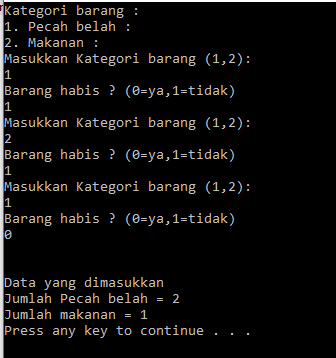
\includegraphics[scale=1]{image6}
\end{center}

\section{Latihan}
\paragraph{Masalah\\}
Modifikasi praktik 1 dengan mengubah bentuk perulangan for menjadi while dan do-while, amati hasilnya, jelaskan dalam laporan
\begin{center}
    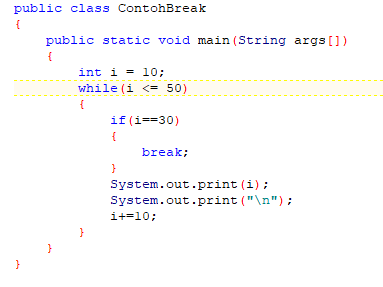
\includegraphics[scale=1]{image7}
\end{center}
untuk mengubah program menjadi perulangan while seperti di atas, maka variabel i yang diperlukan untuk perulangan dideklarasikan terlebih dahulu, lalu perulangan while diberi kondisi yang sama yaitu i <= 50, lalu di akhir pernyataan di perulangan ini diberi i+=10, yaitu variabel i akan ditambah 10 disetiap perulangan, sehingga perulangan ini dapat berhenti. Output program setelah perulangannya dirubah menjadi while adalah sebagai berikut.
\begin{center}
    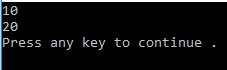
\includegraphics[scale=1]{image8}
\end{center}
\begin{center}
    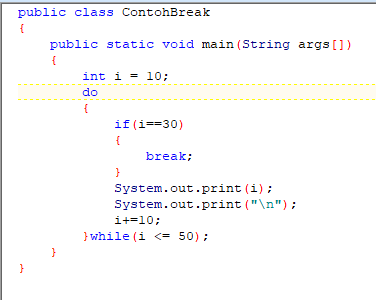
\includegraphics[scale=1]{image9}
\end{center}
Sedangkan jika program dirubah menjadi do-while, yang diperlukan hanyalah menambahkan do di program yang sudah dirubah menjadi while tadi, dan memindahkan while ke akhir statement perulangan, output programnya seperti berikut.
\begin{center}
    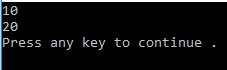
\includegraphics[scale=1]{image10}
\end{center}

\section{Tugas}
\begin{center}
    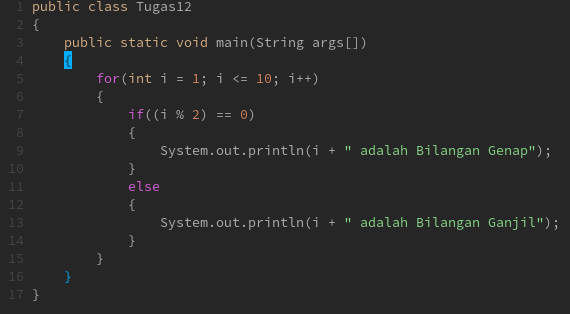
\includegraphics[scale=.8]{image11}
\end{center}
Program di atas memiliki perulangan for, yang akan menghitung bilangan dari 1 sampai 10, lalu didalamnya terdapat seleksi if, jika modulo variabel i sama dengan 0 jika dibagi dengan 2, maka program akan menambahkan " adalah bilangan genap" namun jika tidak maka akan menambahkan " adalah bilangan ganjil". Jadi program ini akan menghitung 1 - 10 dan menyatakan antara bilangan genap dan ganjil. Jadi outputnya seperti berikut.
\begin{center}
    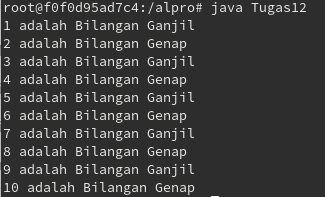
\includegraphics[scale=1]{image12}
\end{center}

\newpage
\section{Kesimpulan}
Mahasiswa dapat mengimplementasikan konsep perulangan while untuk menyelesaikan kasus


\end{document}
